\documentclass[a4paper]{report}
\usepackage[fontsize=13pt]{scrextend}
\usepackage[style=ieee,sorting=none]{biblatex} %Imports biblatex package
\AtEveryBibitem{%
  \clearfield{issn} % Remove issn
  \clearfield{doi} % Remove doi

  \ifentrytype{online}{}{% Remove url except for @online
    \clearfield{url}
  }
}
\addbibresource{refs.bib}
\usepackage{longtable}
\usepackage{amsmath}
%new packet added
\usepackage{indentfirst}
\usepackage{ragged2e}
\usepackage{blindtext}
\usepackage{titlesec}
%new packet added
\usepackage{a4wide,amssymb,epsfig,latexsym,multicol,array,hhline,fancyhdr}
\usepackage{vntex}
\usepackage[english]{babel}
\usepackage{mathptmx}[ptm]
\usepackage[normalem]{ulem}
\usepackage{amsmath}
\usepackage{lastpage}
\usepackage[lined,boxed,commentsnumbered]{algorithm2e}
\usepackage{enumerate}
\usepackage{color}
\usepackage{graphicx}							% Standard graphics package
\usepackage{array}
\usepackage{tabularx}
\usepackage{caption}
\usepackage{multirow}
\usepackage{multicol}
\usepackage{rotating}
\usepackage{graphics}
\usepackage{geometry}
\usepackage{setspace}
\usepackage{epsfig}
\usepackage{tikz}
\usepackage{subcaption}
\usepackage{longfbox}
\usepackage{float}
\usepackage{pdfpages}

\usetikzlibrary{arrows,snakes,backgrounds,calc}
\usepackage{hyperref}
\hypersetup{urlcolor=blue,linkcolor=black,citecolor=black,colorlinks=true} 
\usepackage{comment}
\usepackage{tocloft}
\usepackage{appendix}
% \usepackage{algorithm2e}
\usepackage{algorithm}
\usepackage{algorithmic}
\renewcommand{\algorithmicrequire}{\textbf{Input:}}
\renewcommand{\algorithmicensure}{\textbf{Output:}}

\RestyleAlgo{ruled}

\SetKwComment{Comment}{/* }{ */}

\DeclareMathAlphabet{\mathcal}{OMS}{cmsy}{m}{n}

% \renewcommand{\cftfigindent}{pt}
\renewcommand{\cftfigpresnum}{\figurename~}
\renewcommand{\cftfignumwidth}{5em}

% \renewcommand{\cfttabindent}{0.5pt}
\renewcommand{\cfttabpresnum}{\tablename~}
\renewcommand{\cfttabnumwidth}{5em}
\newtheorem{theorem}{{\bf Theorem}}
\newtheorem{property}{{\bf Property}}
\newtheorem{proposition}{{\bf Proposition}}
\newtheorem{corollary}[proposition]{{\bf Corollary}}
\newtheorem{lemma}[proposition]{{\bf Lemma}}

%%%Setting document
\renewcommand{\baselinestretch}{1.5} 

\def\thesislayout{	% A4: 210 × 297
	\newgeometry{
		a4paper,
		total={210mm,297mm},  % fix over page
		left=35mm,
		top=25mm,
            bottom=30mm,
            right=30mm
	}
}
\def\thesisheadlayout{	% A4: 210 × 297
	\geometry{
		a4paper,
		total={210mm,297mm},  % fix over page
		left=40mm,
		top=30mm,
            bottom=30mm,
            right=30mm
	}
}
\AtBeginDocument{\renewcommand*\contentsname{Contents}}
\AtBeginDocument{\renewcommand*\refname{References}}

\thesisheadlayout
%\usepackage{fancyhdr}
\setlength{\headheight}{40pt}
% \pagestyle{fancy}
% \fancyhead{} % clear all header fields
% \fancyhead[L]{
%  \begin{tabular}{rl}
%     \begin{picture}(25,15)(0,0)
%     \put(0,-8){
\includegraphics[width=8mm, height=8mm]{image/hcmut.png}}
%     %\put(0,-8){\epsfig{width=10mm,figure=hcmut.eps}}
%    \end{picture}&
% 	%
\includegraphics[width=8mm, height=8mm]{hcmut.png} & %
% 	\begin{tabular}{l}
% 		\textbf{\bf Ho Chi Minh City University of Technology}\\
% 		\textbf{\bf  Faculty of Computer Science and Engineering}
% 	\end{tabular} 	
%  \end{tabular}
% }
% \fancyhead[R]{
% 	\begin{tabular}{l}
% 		\tiny \bf \\
% 		\tiny \bf 
% 	\end{tabular}  }
\fancyfoot{} % clear all footer fields
% \fancyfoot[L]{\scriptsize  Specialized Project Report (CO3335) - Semester-231 2023 - 2024}
\fancyfoot[R]{\scriptsize Page {\thepage}/\pageref{LastPage}}
\renewcommand{\headrulewidth}{0.3pt}
\renewcommand{\footrulewidth}{0.3pt}

\setlength\parindent{0pt}
%%%
\setcounter{secnumdepth}{4}
\setcounter{tocdepth}{3}
\makeatletter
\newcounter {subsubsubsection}[subsubsection]
\renewcommand\thesubsubsubsection{\thesubsubsection .\@alph\c@subsubsubsection}
\newcommand\subsubsubsection{\@startsection{subsubsubsection}{4}{\z@}%
                                     {-3.25ex\@plus -1ex \@minus -.2ex}%
                                     {1.5ex \@plus .2ex}%
                                     {\normalfont\normalsize\bfseries}}
\newcommand*\l@subsubsubsection{\@dottedtocline{3}{10.0em}{4.1em}}
\newcommand*{\subsubsubsectionmark}[1]{}
\newcommand\tab[1][1cm]{\hspace*{#1}}
\newcommand\blank[1]{\rule[-.2ex]{#1}{.4pt}}
\makeatother
% \usepackage{longtable}

\newcounter{tmp}
\newcommand\tabularhead[1]{
% \begin{table}[h]
  \begin{longtable}{|p{0.3\linewidth}|p{0.55\linewidth}|}
  \caption{Use-case #1}
    
    \hline
    \textbf{Use-case} & {\textbf{#1}} \\
    \hline}

  \newcommand\addrow[2]{#1 & #2 \\ \hline}

  \newcommand\addmulrow[2]{ #1 
     &  \begin{enumerate} #2  \setcounter{tmp}{\value{enumi}}\end{enumerate}  \\ \hline}
     
  \newcommand\addbreakmulrow[1]{ 
     &  \begin{enumerate}\setcounter{enumi}{\value{tmp}} #1  \end{enumerate}  \\ \hline}
  
 
  \newenvironment{usecase}{\tabularhead}
{\end{longtable}}
% \end{table}}
\setlength{\floatsep}{5pt plus 2pt minus 2pt}
\setlength{\textfloatsep}{5pt plus 2pt minus 2pt}
\setlength{\intextsep}{10pt plus 2pt minus 2pt}

\titleformat{\chapter}[display]
{\normalfont\huge\bfseries}{\chaptertitlename{} \thechapter}{15pt}{\Huge}
\begin{document}

\begin{titlepage}
\begin{tikzpicture}[remember picture, overlay]
  \draw[line width = 4pt] ($(current page.north west) + (30mm,-0.5in)$) rectangle ($(current page.south east) + (-20mm,0.5in)$);
  \draw[line width=1.5pt]
    ($ (current page.north west) + (30mm+0.05in,-0.55in) $)
    rectangle
    ($ (current page.south east) + (-20mm-0.05in,0.55in) $);
\end{tikzpicture}
\vspace{-2.cm}
\begin{center}
\large \textbf{\fontsize{14pt}{0pt}\selectfont VIETNAM NATIONAL UNIVERSITY, HO CHI MINH CITY} \\
\Large \textbf{\fontsize{14pt}{0pt}\selectfont HO CHI MINH CITY UNIVERSITY OF TECHNOLOGY} \\
\Large \textbf{\fontsize{14pt}{0pt}\selectfont FACULTY OF COMPUTER SCIENCE AND ENGINEERING}
\end{center}

\vspace{0.3cm}

\begin{figure}[h!]
\begin{center}

\includegraphics[width=8cm]{image/hcmut.png}
\end{center}
\end{figure}
\vspace{-1cm}
\begin{center}
\begin{tabular}{c}
\multicolumn{1}{c}{\textbf{{\Large REPORT}}}
\\{\textbf{{\Large \MakeUppercase{CAPSTONE PROJECT}}}}
\\

\end{tabular}
\end{center}
% Title
\rule[0.4cm]{\linewidth}{0.3mm} 
\centering
{\Large \bfseries \MakeUppercase{Large Language Model Knowledge Enhancement With Retrieval Augmentation}}    

\rule{\linewidth}{0.2mm} \\[0.1cm]
\begin{center}
    \MakeUppercase{\textbf{\Large Major: \Large Computer Science}}
\end{center}

\vspace{0.01cm}

\begin{center}
\begin{tabular}[H]{r l l}
     \large \textbf{THESIS COMMITTEE} &: \large COMPUTER SCIENCE - CLC 01\\
     \large \textbf{SUPERVISOR(s)} & : \large QUAN THANH THO, Ph.D.\\
                                    & : \large NGUYEN QUANG DUC, B.Eng.\\
     \large \textbf{REVIEWER} & : \large VO THANH HUNG, M.Eng.\\
     \multicolumn{2}{c}{\textbf{\large ————o0o———–}}\\
     \large \textbf{STUDENT}& : \large LE DUC DONG - 2052450\\
   
\end{tabular}    
\end{center}
\vspace{1.cm}
\begin{center}
{\fontsize{12pt}{0pt} HO CHI MINH CITY, May 2024}
\end{center}
\end{titlepage}

% \thesislayout

%\thispagestyle{empty}
\renewcommand{\figurename}{\textbf{Figure}}
\renewcommand{\tablename}{\textbf{Table}}
\newpage

%%%%%%%%%%%%%%%%%%%%%%%%%%%%%%%%%
\pagenumbering{roman}

% \section*{\Huge Abstract}
Large Language Models (LLMs) have revolutionized natural language processing, showcasing remarkable capabilities in tasks such as text generation, translation, and question answering. However, their reliance on massive text datasets for training often results in factual inaccuracies, inconsistencies, and limitations in accessing specific knowledge domains. This inherent constraint hinders their performance in scenarios demanding precise factual accuracy and comprehensive knowledge retrieval. To address these challenges, this project explores the integration of knowledge graphs, structured representations of information, with LLMs. We analyze existing retrieval-augmented generation (RAG) techniques, including Text-Based RAG, which retrieves relevant documents from external corpora, and Knowledge Graph-Based RAG (KG-RAG), which leverages knowledge graph information to enrich LLM responses. While these methods demonstrate improvements, they often suffer from retrieval bottlenecks and challenges in incorporating external knowledge into the LLM's reasoning process. To overcome these limitations, we propose KEALLM - a Knowledge Graph Embedding Augmented Large Language Model. Unlike other RAG approaches, KEALLM directly incorporates knowledge graph embeddings into the LLM architecture, enabling a more integrated and efficient knowledge utilization. To evaluate the effectiveness of KEALLM, we conduct experiments on one-hop question answering tasks, comparing its performance against standard LLMs, Text-Based RAG, and KG-RAG. Our results demonstrate that KEALLM consistently outperforms standard LLMs and Text-Based RAG, achieving comparable performance to KG-RAG while offering a more streamlined and efficient architecture. This project highlights the significant potential of integrating knowledge graph embeddings with LLMs. KEALLM offers a promising avenue for developing more knowledgeable, accurate, and reliable LLMs, paving the way for advancements in various domains, including question answering, dialogue systems, and knowledge-intensive Natural Language Processing (NLP) applications. Further research will focus on refining KEALLM's architecture, exploring different knowledge graph embedding techniques, and evaluating its performance on more complex NLP tasks.

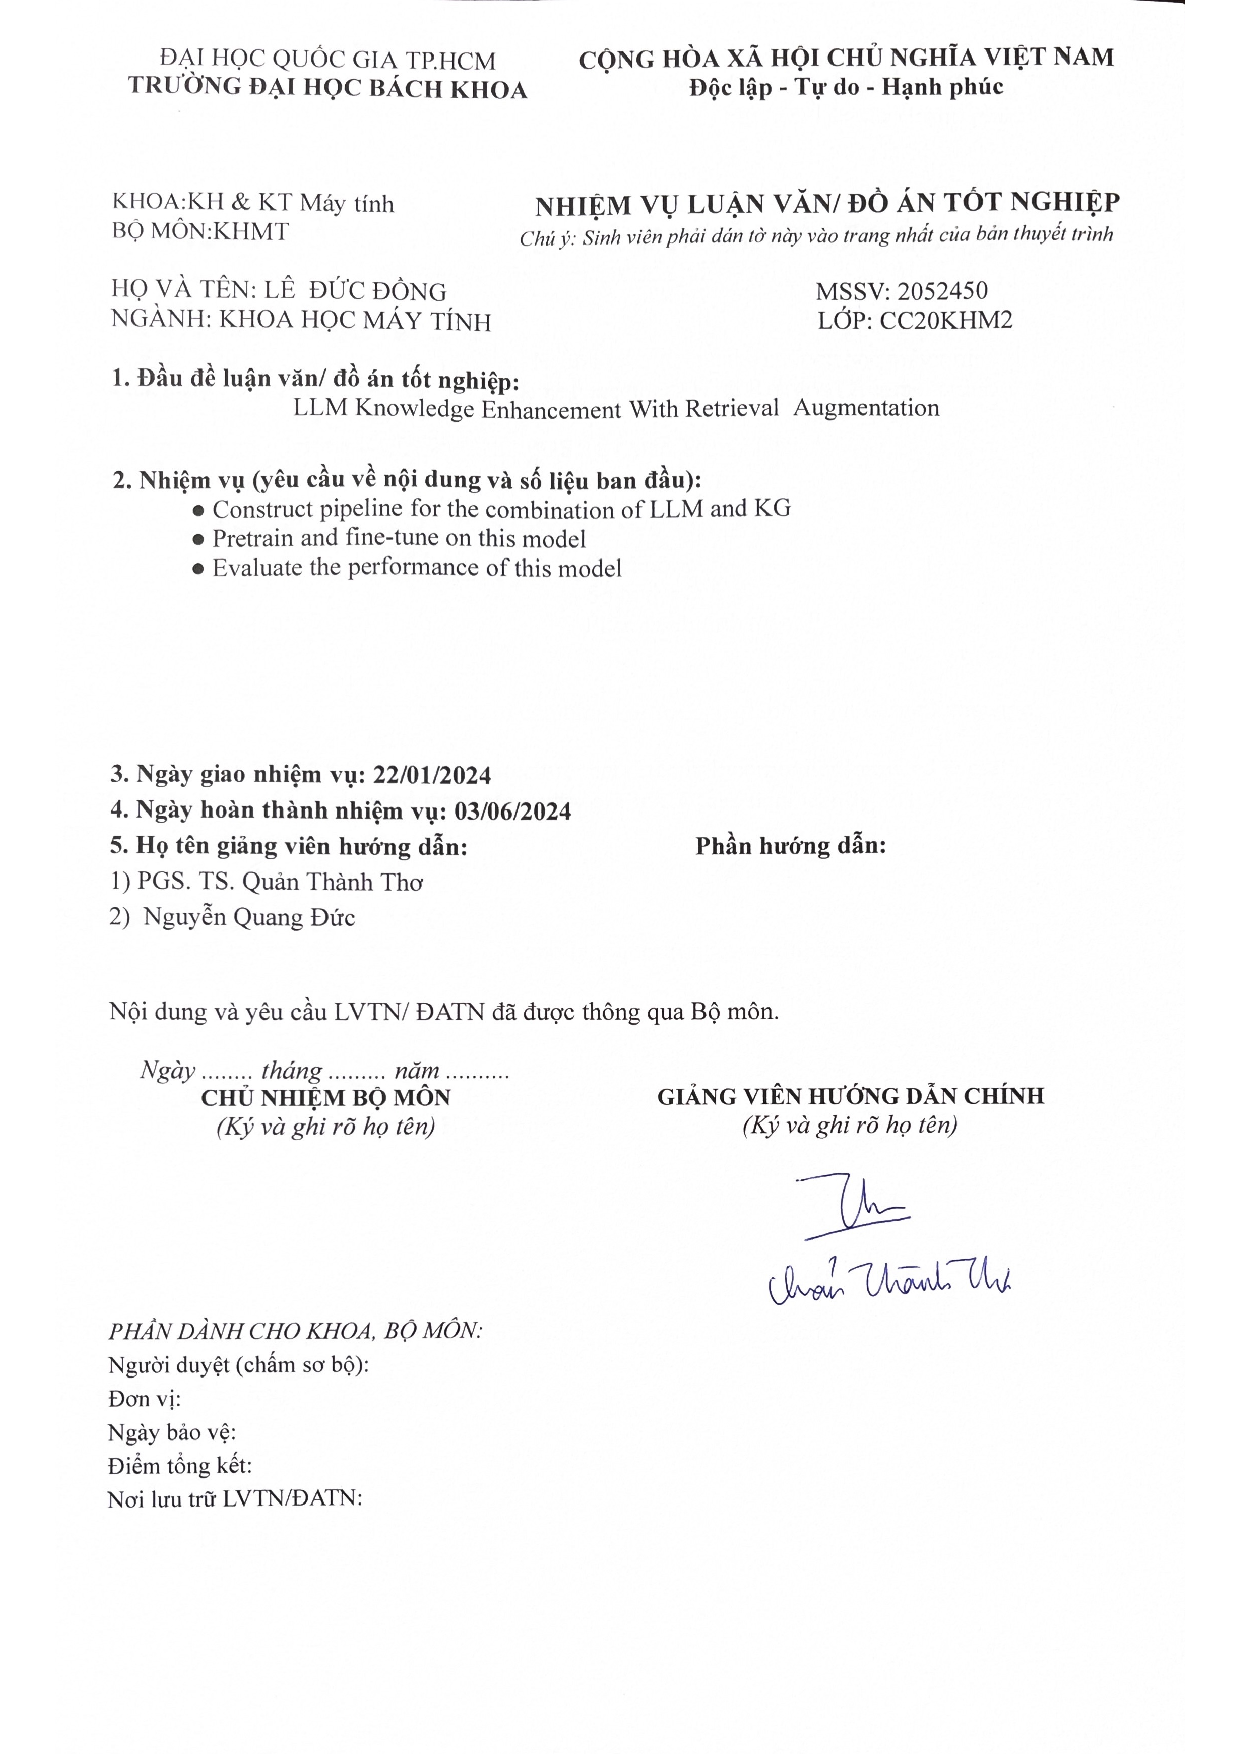
\includepdf[pages=-]{instructor-signature/task.pdf}
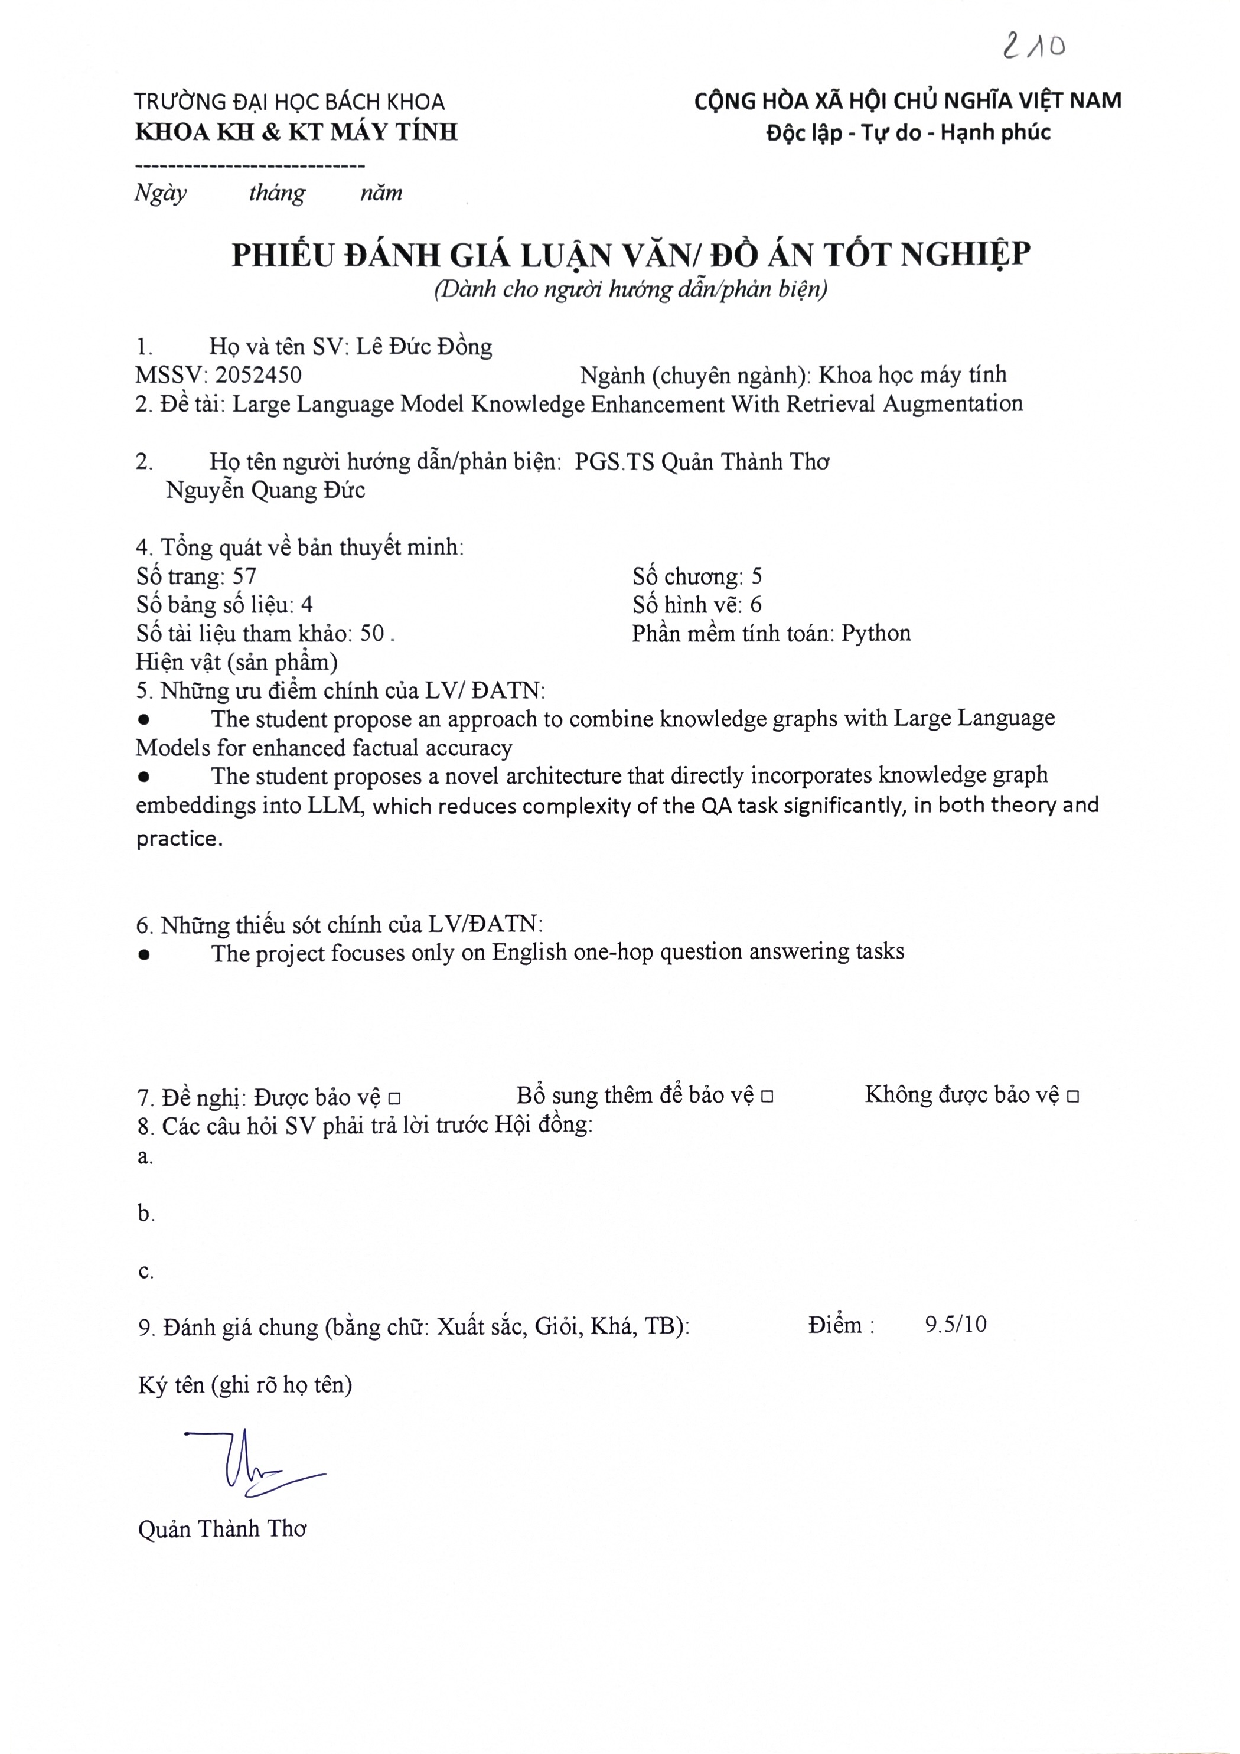
\includepdf[pages=-]{instructor-signature/Dong.pdf}
\setcounter{page}{1}
\section*{\Huge Abstract}
Large Language Models (LLMs) have revolutionized natural language processing, showcasing remarkable capabilities in tasks such as text generation, translation, and question answering. However, their reliance on massive text datasets for training often results in factual inaccuracies, inconsistencies, and limitations in accessing specific knowledge domains. This inherent constraint hinders their performance in scenarios demanding precise factual accuracy and comprehensive knowledge retrieval. To address these challenges, this project explores the integration of knowledge graphs, structured representations of information, with LLMs. We analyze existing retrieval-augmented generation (RAG) techniques, including Text-Based RAG, which retrieves relevant documents from external corpora, and Knowledge Graph-Based RAG (KG-RAG), which leverages knowledge graph information to enrich LLM responses. While these methods demonstrate improvements, they often suffer from retrieval bottlenecks and challenges in incorporating external knowledge into the LLM's reasoning process. To overcome these limitations, we propose KEALLM - a Knowledge Graph Embedding Augmented Large Language Model. Unlike other RAG approaches, KEALLM directly incorporates knowledge graph embeddings into the LLM architecture, enabling a more integrated and efficient knowledge utilization. To evaluate the effectiveness of KEALLM, we conduct experiments on one-hop question answering tasks, comparing its performance against standard LLMs, Text-Based RAG, and KG-RAG. Our results demonstrate that KEALLM consistently outperforms standard LLMs and Text-Based RAG, achieving comparable performance to KG-RAG while offering a more streamlined and efficient architecture. This project highlights the significant potential of integrating knowledge graph embeddings with LLMs. KEALLM offers a promising avenue for developing more knowledgeable, accurate, and reliable LLMs, paving the way for advancements in various domains, including question answering, dialogue systems, and knowledge-intensive Natural Language Processing (NLP) applications. Further research will focus on refining KEALLM's architecture, exploring different knowledge graph embedding techniques, and evaluating its performance on more complex NLP tasks.


\section*{\Huge Abstract}
Large Language Models (LLMs) have revolutionized natural language processing, showcasing remarkable capabilities in tasks such as text generation, translation, and question answering. However, their reliance on massive text datasets for training often results in factual inaccuracies, inconsistencies, and limitations in accessing specific knowledge domains. This inherent constraint hinders their performance in scenarios demanding precise factual accuracy and comprehensive knowledge retrieval. To address these challenges, this project explores the integration of knowledge graphs, structured representations of information, with LLMs. We analyze existing retrieval-augmented generation (RAG) techniques, including Text-Based RAG, which retrieves relevant documents from external corpora, and Knowledge Graph-Based RAG (KG-RAG), which leverages knowledge graph information to enrich LLM responses. While these methods demonstrate improvements, they often suffer from retrieval bottlenecks and challenges in incorporating external knowledge into the LLM's reasoning process. To overcome these limitations, we propose KEALLM - a Knowledge Graph Embedding Augmented Large Language Model. Unlike other RAG approaches, KEALLM directly incorporates knowledge graph embeddings into the LLM architecture, enabling a more integrated and efficient knowledge utilization. To evaluate the effectiveness of KEALLM, we conduct experiments on one-hop question answering tasks, comparing its performance against standard LLMs, Text-Based RAG, and KG-RAG. Our results demonstrate that KEALLM consistently outperforms standard LLMs and Text-Based RAG, achieving comparable performance to KG-RAG while offering a more streamlined and efficient architecture. This project highlights the significant potential of integrating knowledge graph embeddings with LLMs. KEALLM offers a promising avenue for developing more knowledgeable, accurate, and reliable LLMs, paving the way for advancements in various domains, including question answering, dialogue systems, and knowledge-intensive Natural Language Processing (NLP) applications. Further research will focus on refining KEALLM's architecture, exploring different knowledge graph embedding techniques, and evaluating its performance on more complex NLP tasks.


\section*{\Huge Abstract}
Large Language Models (LLMs) have revolutionized natural language processing, showcasing remarkable capabilities in tasks such as text generation, translation, and question answering. However, their reliance on massive text datasets for training often results in factual inaccuracies, inconsistencies, and limitations in accessing specific knowledge domains. This inherent constraint hinders their performance in scenarios demanding precise factual accuracy and comprehensive knowledge retrieval. To address these challenges, this project explores the integration of knowledge graphs, structured representations of information, with LLMs. We analyze existing retrieval-augmented generation (RAG) techniques, including Text-Based RAG, which retrieves relevant documents from external corpora, and Knowledge Graph-Based RAG (KG-RAG), which leverages knowledge graph information to enrich LLM responses. While these methods demonstrate improvements, they often suffer from retrieval bottlenecks and challenges in incorporating external knowledge into the LLM's reasoning process. To overcome these limitations, we propose KEALLM - a Knowledge Graph Embedding Augmented Large Language Model. Unlike other RAG approaches, KEALLM directly incorporates knowledge graph embeddings into the LLM architecture, enabling a more integrated and efficient knowledge utilization. To evaluate the effectiveness of KEALLM, we conduct experiments on one-hop question answering tasks, comparing its performance against standard LLMs, Text-Based RAG, and KG-RAG. Our results demonstrate that KEALLM consistently outperforms standard LLMs and Text-Based RAG, achieving comparable performance to KG-RAG while offering a more streamlined and efficient architecture. This project highlights the significant potential of integrating knowledge graph embeddings with LLMs. KEALLM offers a promising avenue for developing more knowledgeable, accurate, and reliable LLMs, paving the way for advancements in various domains, including question answering, dialogue systems, and knowledge-intensive Natural Language Processing (NLP) applications. Further research will focus on refining KEALLM's architecture, exploring different knowledge graph embedding techniques, and evaluating its performance on more complex NLP tasks.


%%%%%%%%%%%%%%%%%%%%%%%%%%%%%%%%%
\tableofcontents
\newpage
\listoffigures
\newpage
\listoftables
\newpage
%%%%%%%%%%%%%%%%%%%%%%%%%%%%%%%%%
\pagenumbering{arabic}
\setcounter{page}{1}
\thesislayout
\section*{\Huge Abstract}
Large Language Models (LLMs) have revolutionized natural language processing, showcasing remarkable capabilities in tasks such as text generation, translation, and question answering. However, their reliance on massive text datasets for training often results in factual inaccuracies, inconsistencies, and limitations in accessing specific knowledge domains. This inherent constraint hinders their performance in scenarios demanding precise factual accuracy and comprehensive knowledge retrieval. To address these challenges, this project explores the integration of knowledge graphs, structured representations of information, with LLMs. We analyze existing retrieval-augmented generation (RAG) techniques, including Text-Based RAG, which retrieves relevant documents from external corpora, and Knowledge Graph-Based RAG (KG-RAG), which leverages knowledge graph information to enrich LLM responses. While these methods demonstrate improvements, they often suffer from retrieval bottlenecks and challenges in incorporating external knowledge into the LLM's reasoning process. To overcome these limitations, we propose KEALLM - a Knowledge Graph Embedding Augmented Large Language Model. Unlike other RAG approaches, KEALLM directly incorporates knowledge graph embeddings into the LLM architecture, enabling a more integrated and efficient knowledge utilization. To evaluate the effectiveness of KEALLM, we conduct experiments on one-hop question answering tasks, comparing its performance against standard LLMs, Text-Based RAG, and KG-RAG. Our results demonstrate that KEALLM consistently outperforms standard LLMs and Text-Based RAG, achieving comparable performance to KG-RAG while offering a more streamlined and efficient architecture. This project highlights the significant potential of integrating knowledge graph embeddings with LLMs. KEALLM offers a promising avenue for developing more knowledgeable, accurate, and reliable LLMs, paving the way for advancements in various domains, including question answering, dialogue systems, and knowledge-intensive Natural Language Processing (NLP) applications. Further research will focus on refining KEALLM's architecture, exploring different knowledge graph embedding techniques, and evaluating its performance on more complex NLP tasks.

\section*{\Huge Abstract}
Large Language Models (LLMs) have revolutionized natural language processing, showcasing remarkable capabilities in tasks such as text generation, translation, and question answering. However, their reliance on massive text datasets for training often results in factual inaccuracies, inconsistencies, and limitations in accessing specific knowledge domains. This inherent constraint hinders their performance in scenarios demanding precise factual accuracy and comprehensive knowledge retrieval. To address these challenges, this project explores the integration of knowledge graphs, structured representations of information, with LLMs. We analyze existing retrieval-augmented generation (RAG) techniques, including Text-Based RAG, which retrieves relevant documents from external corpora, and Knowledge Graph-Based RAG (KG-RAG), which leverages knowledge graph information to enrich LLM responses. While these methods demonstrate improvements, they often suffer from retrieval bottlenecks and challenges in incorporating external knowledge into the LLM's reasoning process. To overcome these limitations, we propose KEALLM - a Knowledge Graph Embedding Augmented Large Language Model. Unlike other RAG approaches, KEALLM directly incorporates knowledge graph embeddings into the LLM architecture, enabling a more integrated and efficient knowledge utilization. To evaluate the effectiveness of KEALLM, we conduct experiments on one-hop question answering tasks, comparing its performance against standard LLMs, Text-Based RAG, and KG-RAG. Our results demonstrate that KEALLM consistently outperforms standard LLMs and Text-Based RAG, achieving comparable performance to KG-RAG while offering a more streamlined and efficient architecture. This project highlights the significant potential of integrating knowledge graph embeddings with LLMs. KEALLM offers a promising avenue for developing more knowledgeable, accurate, and reliable LLMs, paving the way for advancements in various domains, including question answering, dialogue systems, and knowledge-intensive Natural Language Processing (NLP) applications. Further research will focus on refining KEALLM's architecture, exploring different knowledge graph embedding techniques, and evaluating its performance on more complex NLP tasks.

\section*{\Huge Abstract}
Large Language Models (LLMs) have revolutionized natural language processing, showcasing remarkable capabilities in tasks such as text generation, translation, and question answering. However, their reliance on massive text datasets for training often results in factual inaccuracies, inconsistencies, and limitations in accessing specific knowledge domains. This inherent constraint hinders their performance in scenarios demanding precise factual accuracy and comprehensive knowledge retrieval. To address these challenges, this project explores the integration of knowledge graphs, structured representations of information, with LLMs. We analyze existing retrieval-augmented generation (RAG) techniques, including Text-Based RAG, which retrieves relevant documents from external corpora, and Knowledge Graph-Based RAG (KG-RAG), which leverages knowledge graph information to enrich LLM responses. While these methods demonstrate improvements, they often suffer from retrieval bottlenecks and challenges in incorporating external knowledge into the LLM's reasoning process. To overcome these limitations, we propose KEALLM - a Knowledge Graph Embedding Augmented Large Language Model. Unlike other RAG approaches, KEALLM directly incorporates knowledge graph embeddings into the LLM architecture, enabling a more integrated and efficient knowledge utilization. To evaluate the effectiveness of KEALLM, we conduct experiments on one-hop question answering tasks, comparing its performance against standard LLMs, Text-Based RAG, and KG-RAG. Our results demonstrate that KEALLM consistently outperforms standard LLMs and Text-Based RAG, achieving comparable performance to KG-RAG while offering a more streamlined and efficient architecture. This project highlights the significant potential of integrating knowledge graph embeddings with LLMs. KEALLM offers a promising avenue for developing more knowledgeable, accurate, and reliable LLMs, paving the way for advancements in various domains, including question answering, dialogue systems, and knowledge-intensive Natural Language Processing (NLP) applications. Further research will focus on refining KEALLM's architecture, exploring different knowledge graph embedding techniques, and evaluating its performance on more complex NLP tasks.

\section*{\Huge Abstract}
Large Language Models (LLMs) have revolutionized natural language processing, showcasing remarkable capabilities in tasks such as text generation, translation, and question answering. However, their reliance on massive text datasets for training often results in factual inaccuracies, inconsistencies, and limitations in accessing specific knowledge domains. This inherent constraint hinders their performance in scenarios demanding precise factual accuracy and comprehensive knowledge retrieval. To address these challenges, this project explores the integration of knowledge graphs, structured representations of information, with LLMs. We analyze existing retrieval-augmented generation (RAG) techniques, including Text-Based RAG, which retrieves relevant documents from external corpora, and Knowledge Graph-Based RAG (KG-RAG), which leverages knowledge graph information to enrich LLM responses. While these methods demonstrate improvements, they often suffer from retrieval bottlenecks and challenges in incorporating external knowledge into the LLM's reasoning process. To overcome these limitations, we propose KEALLM - a Knowledge Graph Embedding Augmented Large Language Model. Unlike other RAG approaches, KEALLM directly incorporates knowledge graph embeddings into the LLM architecture, enabling a more integrated and efficient knowledge utilization. To evaluate the effectiveness of KEALLM, we conduct experiments on one-hop question answering tasks, comparing its performance against standard LLMs, Text-Based RAG, and KG-RAG. Our results demonstrate that KEALLM consistently outperforms standard LLMs and Text-Based RAG, achieving comparable performance to KG-RAG while offering a more streamlined and efficient architecture. This project highlights the significant potential of integrating knowledge graph embeddings with LLMs. KEALLM offers a promising avenue for developing more knowledgeable, accurate, and reliable LLMs, paving the way for advancements in various domains, including question answering, dialogue systems, and knowledge-intensive Natural Language Processing (NLP) applications. Further research will focus on refining KEALLM's architecture, exploring different knowledge graph embedding techniques, and evaluating its performance on more complex NLP tasks.

\section*{\Huge Abstract}
Large Language Models (LLMs) have revolutionized natural language processing, showcasing remarkable capabilities in tasks such as text generation, translation, and question answering. However, their reliance on massive text datasets for training often results in factual inaccuracies, inconsistencies, and limitations in accessing specific knowledge domains. This inherent constraint hinders their performance in scenarios demanding precise factual accuracy and comprehensive knowledge retrieval. To address these challenges, this project explores the integration of knowledge graphs, structured representations of information, with LLMs. We analyze existing retrieval-augmented generation (RAG) techniques, including Text-Based RAG, which retrieves relevant documents from external corpora, and Knowledge Graph-Based RAG (KG-RAG), which leverages knowledge graph information to enrich LLM responses. While these methods demonstrate improvements, they often suffer from retrieval bottlenecks and challenges in incorporating external knowledge into the LLM's reasoning process. To overcome these limitations, we propose KEALLM - a Knowledge Graph Embedding Augmented Large Language Model. Unlike other RAG approaches, KEALLM directly incorporates knowledge graph embeddings into the LLM architecture, enabling a more integrated and efficient knowledge utilization. To evaluate the effectiveness of KEALLM, we conduct experiments on one-hop question answering tasks, comparing its performance against standard LLMs, Text-Based RAG, and KG-RAG. Our results demonstrate that KEALLM consistently outperforms standard LLMs and Text-Based RAG, achieving comparable performance to KG-RAG while offering a more streamlined and efficient architecture. This project highlights the significant potential of integrating knowledge graph embeddings with LLMs. KEALLM offers a promising avenue for developing more knowledgeable, accurate, and reliable LLMs, paving the way for advancements in various domains, including question answering, dialogue systems, and knowledge-intensive Natural Language Processing (NLP) applications. Further research will focus on refining KEALLM's architecture, exploring different knowledge graph embedding techniques, and evaluating its performance on more complex NLP tasks.

% \section*{\Huge Abstract}
Large Language Models (LLMs) have revolutionized natural language processing, showcasing remarkable capabilities in tasks such as text generation, translation, and question answering. However, their reliance on massive text datasets for training often results in factual inaccuracies, inconsistencies, and limitations in accessing specific knowledge domains. This inherent constraint hinders their performance in scenarios demanding precise factual accuracy and comprehensive knowledge retrieval. To address these challenges, this project explores the integration of knowledge graphs, structured representations of information, with LLMs. We analyze existing retrieval-augmented generation (RAG) techniques, including Text-Based RAG, which retrieves relevant documents from external corpora, and Knowledge Graph-Based RAG (KG-RAG), which leverages knowledge graph information to enrich LLM responses. While these methods demonstrate improvements, they often suffer from retrieval bottlenecks and challenges in incorporating external knowledge into the LLM's reasoning process. To overcome these limitations, we propose KEALLM - a Knowledge Graph Embedding Augmented Large Language Model. Unlike other RAG approaches, KEALLM directly incorporates knowledge graph embeddings into the LLM architecture, enabling a more integrated and efficient knowledge utilization. To evaluate the effectiveness of KEALLM, we conduct experiments on one-hop question answering tasks, comparing its performance against standard LLMs, Text-Based RAG, and KG-RAG. Our results demonstrate that KEALLM consistently outperforms standard LLMs and Text-Based RAG, achieving comparable performance to KG-RAG while offering a more streamlined and efficient architecture. This project highlights the significant potential of integrating knowledge graph embeddings with LLMs. KEALLM offers a promising avenue for developing more knowledgeable, accurate, and reliable LLMs, paving the way for advancements in various domains, including question answering, dialogue systems, and knowledge-intensive Natural Language Processing (NLP) applications. Further research will focus on refining KEALLM's architecture, exploring different knowledge graph embedding techniques, and evaluating its performance on more complex NLP tasks.

% \newpage
% \newpage
% \section*{\Huge Abstract}
Large Language Models (LLMs) have revolutionized natural language processing, showcasing remarkable capabilities in tasks such as text generation, translation, and question answering. However, their reliance on massive text datasets for training often results in factual inaccuracies, inconsistencies, and limitations in accessing specific knowledge domains. This inherent constraint hinders their performance in scenarios demanding precise factual accuracy and comprehensive knowledge retrieval. To address these challenges, this project explores the integration of knowledge graphs, structured representations of information, with LLMs. We analyze existing retrieval-augmented generation (RAG) techniques, including Text-Based RAG, which retrieves relevant documents from external corpora, and Knowledge Graph-Based RAG (KG-RAG), which leverages knowledge graph information to enrich LLM responses. While these methods demonstrate improvements, they often suffer from retrieval bottlenecks and challenges in incorporating external knowledge into the LLM's reasoning process. To overcome these limitations, we propose KEALLM - a Knowledge Graph Embedding Augmented Large Language Model. Unlike other RAG approaches, KEALLM directly incorporates knowledge graph embeddings into the LLM architecture, enabling a more integrated and efficient knowledge utilization. To evaluate the effectiveness of KEALLM, we conduct experiments on one-hop question answering tasks, comparing its performance against standard LLMs, Text-Based RAG, and KG-RAG. Our results demonstrate that KEALLM consistently outperforms standard LLMs and Text-Based RAG, achieving comparable performance to KG-RAG while offering a more streamlined and efficient architecture. This project highlights the significant potential of integrating knowledge graph embeddings with LLMs. KEALLM offers a promising avenue for developing more knowledgeable, accurate, and reliable LLMs, paving the way for advancements in various domains, including question answering, dialogue systems, and knowledge-intensive Natural Language Processing (NLP) applications. Further research will focus on refining KEALLM's architecture, exploring different knowledge graph embedding techniques, and evaluating its performance on more complex NLP tasks.

% \newpage

% \nocite{*}
\addcontentsline{toc}{chapter}{References}
\printbibliography[title=References]

\section*{\Huge Abstract}
Large Language Models (LLMs) have revolutionized natural language processing, showcasing remarkable capabilities in tasks such as text generation, translation, and question answering. However, their reliance on massive text datasets for training often results in factual inaccuracies, inconsistencies, and limitations in accessing specific knowledge domains. This inherent constraint hinders their performance in scenarios demanding precise factual accuracy and comprehensive knowledge retrieval. To address these challenges, this project explores the integration of knowledge graphs, structured representations of information, with LLMs. We analyze existing retrieval-augmented generation (RAG) techniques, including Text-Based RAG, which retrieves relevant documents from external corpora, and Knowledge Graph-Based RAG (KG-RAG), which leverages knowledge graph information to enrich LLM responses. While these methods demonstrate improvements, they often suffer from retrieval bottlenecks and challenges in incorporating external knowledge into the LLM's reasoning process. To overcome these limitations, we propose KEALLM - a Knowledge Graph Embedding Augmented Large Language Model. Unlike other RAG approaches, KEALLM directly incorporates knowledge graph embeddings into the LLM architecture, enabling a more integrated and efficient knowledge utilization. To evaluate the effectiveness of KEALLM, we conduct experiments on one-hop question answering tasks, comparing its performance against standard LLMs, Text-Based RAG, and KG-RAG. Our results demonstrate that KEALLM consistently outperforms standard LLMs and Text-Based RAG, achieving comparable performance to KG-RAG while offering a more streamlined and efficient architecture. This project highlights the significant potential of integrating knowledge graph embeddings with LLMs. KEALLM offers a promising avenue for developing more knowledgeable, accurate, and reliable LLMs, paving the way for advancements in various domains, including question answering, dialogue systems, and knowledge-intensive Natural Language Processing (NLP) applications. Further research will focus on refining KEALLM's architecture, exploring different knowledge graph embedding techniques, and evaluating its performance on more complex NLP tasks.

\end{document}
